\documentclass[a4paper,11pt]{article}

\usepackage{lmodern}
\usepackage[T1]{fontenc}      %font
\usepackage[swedish]{babel}   %svenska
\usepackage[utf8]{inputenc}   %svenska åäö
\usepackage{lr-cover}         %förstasidan
\usepackage{lipsum}           %onödiga texten
\usepackage{booktabs}         %referat
\usepackage{amsmath, amssymb, upref} %matte
\usepackage{amsthm}           %omgivningar
\usepackage{tikz}             %rita i Tikz
\usepackage{caption}
\usepackage{subcaption}
\usetikzlibrary{arrows}       %pilar i Tikz
\usetikzlibrary{calc}         %matte i Tikz
\usetikzlibrary{plotmarks}    %dots i Tikz
\usetikzlibrary{shapes}				%former i Tikz
\usetikzlibrary{plotmarks}    %nått random i Tikz
\usepackage{tocbibind}        %till referenser i innehållsförteckning
\usepackage{graphicx}         %till programmering?
\usepackage{mdframed}					%för inramning
\usepackage{color}						%för text i färg

\newcommand{\highlightYellow}[1]{\colorbox{yellow}{#1}}
\newcommand{\colorFunction}[1]{\textcolor{blue}{#1}}
\newcommand{\colorType}[1]{\textcolor{violet}{#1}}


\begin{document}

\title{Projekt i Realtid- och Operativsystem}
\author{Tim Nyman, Filip Pentikäinen}
\date{\today}
\maketitle

\begin{abstract}
Laborationen ger till uppgift att laboranterna ska skapa ett simpelt filsystem som kan lagra information i block (bitmaps). Informationen ska sedan kunna skrivas till textfil för att laddas in i ett nytt filsystem. Denna inlämning uppfyller kraven för betyget E.
\end{abstract}

\hskip+1cm	%OBS
\tableofcontents

\section{Inledning}
\subsection{Förberedelse}
Laboranterna fick utföra med flera laborationer för att bekanta sig med Linux-kommandon. 6 timmar föreläsning om filsystem var även tillgängligt.
\subsection{Miljö}
Projektet har skapats på skolans datorer i Linux- och Windows miljö. Då programmet skapar virtuell lagring på primärminnet behöver inte det aktuella filsystemet på datorn vara ett specifikt format.
\subsection{Teori}
Ett filsystem lagrar information över en lång tid på en hårddisk (kallad sekundärminne). Ett filsystem har olika format vilket dikterar hur information lagras. Det finns flera olika format på filsystem med olika fördelar och nackdelar och de kan vara exklusiva till specifika OS. 

Användaren av datorn ska kunna organisera information på det sätt användaren vill, detta kräver att filsystemet ska kunna vara flexibelt i hur användaren ser sina filer och mappar. Sättet som moderna filsystem till persondatorer hanterar detta är att skapa en trädstruktur av mappar och filer som sedan refererar till dess lagrade data på disken. Eftersom all data av filsystemet sparas på samma medium (om inte RAID används) kan man flytta hårddisken till olika datorer utan att filstrukturen ändras. Flera olika filsystem kan användas på samma hårddisk genom partitionering, dock kommer användaren se hårddisken som 2 olika hårddiskar då 2 format på filsystem inte kan kombineras.
\subsection{Resurser}
Ett flertal hjälpfiler var tillgängliga till laboranterna. Dessa var kompilerings- och headerfilerna av block, blockdevice, memblockdevice, filesystem och shell. Dessa filer innehöll den grundläggande strukturen för kommandorutan och allokering av virtuellt minne. 

Flera funktioner som hanterar filers skriv- och läsfunktioner är från början implementerade. Detta gör att det laboranten ska implementera är funktioner som utför grundläggande linux kommandon för mapp- och filhantering. Dessa funktioner ska då hantera blockobjekt för att spara filer. Funktionerna ska även kunna organisera mappar och filer i en trädstruktur som användaren skapar.

\section{Uppgift}
\subsection{Metod}
Då vi endast ville uppfylla kraven för E krävdes det att Linux kommanden cd, mkdir, cp, ls, cat, rm, och pwd skulle implementeras. Kommandot format, som bygger upp ett tomt filsystem, quit, som avslutar programmet, createImage och restoreImage, som sparar och laddar ett filsystem respektive, skulle även implementeras.

Vi implementerade 2 nya klasser; Folder och File. Varje Folder innehåller 2 vektorer, 1 för att hantera de underliggande mapparna och 1 för att hålla reda på de filer som ligger i mappen. Eftersom vi valde att inte använda oss av objekt i mappstrukturen innebär detta att vi inte behöver anropa delete[] när mappar eller filer raderas. Detta gör även att vi kunde använda de specifika vektor-funktionerna för att hantera listorna av mappar och filer. 

Filerna behöver även spara vilket block som håller i deras information, då informationen ska sparas i filsystemet. Detta görs genom att skapa en int array som är lika lång som antalet block i filsystemet och som är fylld med nollor när filsystemet är nytt. Varje array-index representerar ett blocknummer. När en fil ska sparas i ett block så kollar man på denna int array efter ett array-index som innehåller en nolla. Då man hittar denna plats anropar man memblockdevice för att skriva data till samma blocknummer som det array index vi hittade innan. När detta är gjort ändrar man int arrayens index värde från en nolla till en etta, vilket representerar att blocknummret innehåller data som tillhör en fil. Filen sparar även detta nummer för att man ska kunna få tag i filens innehåll av filen. Detta gör att filernas data och mapp- och filstrukturen är helt separata. När man gör en sökning genom mapparnas trädstruktur behöver inte filernas data analyseras i onödan.

Då när en fil raderas med rm -kommandot kommer en funktion kolla vilket blocknummer filen har och byter inte arrayens index värde till en nolla. Det är inte nödvändigt att rensa blocket då när en annan fil vill spara data kommer den skriva över datan som ligger i blocket. Om den nya datan är mindre än den förra datan gör det ingenting för en null-pointer kommer skapas efter den nya datan så när blocket ska läsas läser den inte ut mer data efter denna pekare.
\subsection{Funktioner}
\begin{itemize}
\item \textbf{\colorType{int} \colorFunction{createFile}(\colorType{string} fileName, \colorType{string} content)} \\
Tar in en string som kommer att bli namnet på filen och content som kommer att bli innehållet i filen. Den skapar en char array som vi kopierar in content i följt av symbolen §. Detta är för att enkelt kunna veta hur mycket som är content i blocket. Sedan så söker funktionen efter första lediga blocket genom att kolla vår index-array. När den hittar en ledig plats så sätter den en 1:a i index-arrayen för att markera att det nu finns data i det blocket. Sedan så skapar det en ny fil i filvektorn i mappen currentDir(ectory). Den returnerar en int om det gick bra eller inte som sedan hanteras av shell.

\item \textbf{\colorFunction{removeFile}(\colorType{string} fileName)} \\
Tar in namnet på den filen som man vill ta bort. Sedan så söker den igenom currentDir efter filen man vill ta bort. Om filen inte finns så händer inget. Om den finns så söker den upp var i filvektorn som filen ligger sedan ändrar den platsen i index-arrayen som motsvarar filens id till en 0:a för att markera att platsen är ledig. Sedan så tar vi bort filen från filvektorn.

\item \textbf{\colorFunction{CreateFolder}(\colorType{string} folderName)} \\
Tar in en string som blir namnet på Mappen. Sedan så skapar det en ny mapp i foldervektorn med namnet från string.

\item \textbf{\colorFunction{RemoveFolder}(\colorType{string} folderName)} \\
Tar in namnet på mappen som ska tas bort. Sedan så skapar den en temporär mapp med samma namn för att kunna söka igenom foldervektorn efter en mapp med samma namn. Om den hittar en mapp med samma namn så tar funktionen bort den, annars händer inget.

\item \textbf{\colorType{bool} \colorFunction{GoToFolder}(\colorType{string} folderName)} \\
Tar in en string med namnet på filen vi vill gå till. Sedan så skapar funktionen en char array som den kopierar in strängen i. Om det är en korrekt filepath som matats in så tar den användaren dit. Även om det är flera så fungerar det t.ex “A/A1/A11” och “..” skickar en tillbaka en mapp.

\item \textbf{\colorType{string} \colorFunction{ListContent}()} \\
Denna funktion använder pekaren currentDir för att skriva ut innehållet i den mapp som användaren är i. Funktionen innehåller 2 loopar som först lägger till namnet på alla mappar i användarmappen i en string och sedan lägger på filnamnen efter det. Denna sträng returneras sedan.

\item \textbf{\colorType{string} \colorFunction{PrintFileContent}(\colorType{string} fileName)} \\
Funktionen tar ett filnamn som parameter och letar upp denna i den mapp som användaren befinner sig i. Efter det returneras en sträng med innehållet i filen, som tidigare sparats i ett block av minne. Detta görs genom att använda vektor-funktionen find() för att hitta vilken position i mappens fileVec som filen ligger i. Sedan kollas vilket id filen har och hämtar informationen från samma blocknummer som id:t.

\item \textbf{\colorType{bool} \colorFunction{CopyFile}(\colorType{string} file1, \colorType{string} file2)} \\
Denna funktion tar som parameter 2 filnamn. Funktionen kommer då att hitta en fil i nuvarande mapp med samma namn som file1 och kopiera in dess innehåll i en ny fil med samma namn som file2-parametern. Först hittar vi vilken position i fileVec som file1 har. Sedan kallar vi på funktionen createFile(file2, PrintFileContent(file1)) då denna kommer skapa en ny fil med rätt namn och mata in samma sträng som file1 hade.

\item \textbf{\colorFunction{CreateImage}(\colorType{string} sysName)} \\
Funktionen skapar en textfil med samma namn som sysName och fyller denna med nödvändig data för att bygga upp filsystemet igen. Detta görs med hjälp av funktionen recursiveCreate() som nämns härnest.

\item \textbf{\colorFunction{recursiveCreate}(\colorType{Folder*} dir, \colorType{ofstream} \&file)} \\
Tar en huvudmapp och en textstream som parameter. Från huvudmappen skrivs sedan ut antalet mappar och antalet filer ut till filen. Sedan skrivs alla filers namn ut med dess innehåll därefter delat av ett “=”-tecken. Sedan följer utskrift av mappnamnen och ett anrop av recursiveCreate() efter varje utskrift där den mapp som precis skrivits ut används som parameter.

\item \textbf{\colorFunction{restoreImage}(\colorType{string} filePath)} \\
Funktionen tar som parameter en filväg till en textfil som skapats med CreateImage(). Från denna kommer funktionen återskapa det filsystem som sparats. Funktionen recursiveFunction() för att göra detta, beskrivning av denna följer.

\item \textbf{\colorFunction{restoreImage}(\colorType{Folder*} dir, \colorType{ifstream} \&file)} \\
Tar en huvudmapp som parameter och återställer dess innehåll enligt textfilen som öppnas i restoreImage(). Först återställs mappens filer och sedan dess mappar. Vid varje skapad mapp kallas funktionen restoreImage() igen med den nya mappen som huvudmapp.
\end{itemize}
\subsection{Klassdiagram}
Se Figur 1 för fullständigt klassdiagram. Klassen BlockDevice skapar virtuellt sekundärminne i form av blocks. Dessa block håller 512 byte av data och ska representera en bitmap i en hårddisk. 250 av dessa block skapas av BlockDevice.
MemBlockDevice är en virtuell klass som håller flera funktioner som används i FileSystem-klassen för att hantera blocken i BlockDevice.

FileSystem är klassen där vi har implementerat majoriteten av vår kod. Den innehåller filsystemet med alla mappar som i sin tur innehåller alla filer.

I Shell, där main() befinner sig, skriver användaren in de kommandon som ska utföras av filsystemet. Denna är också ansvarig för att skapa FileSystem som sedan skapar resterande klasser.

\hskip+0.9cm
\begin{figure}[t]
	\begin{center}
		\label{bild_1}
		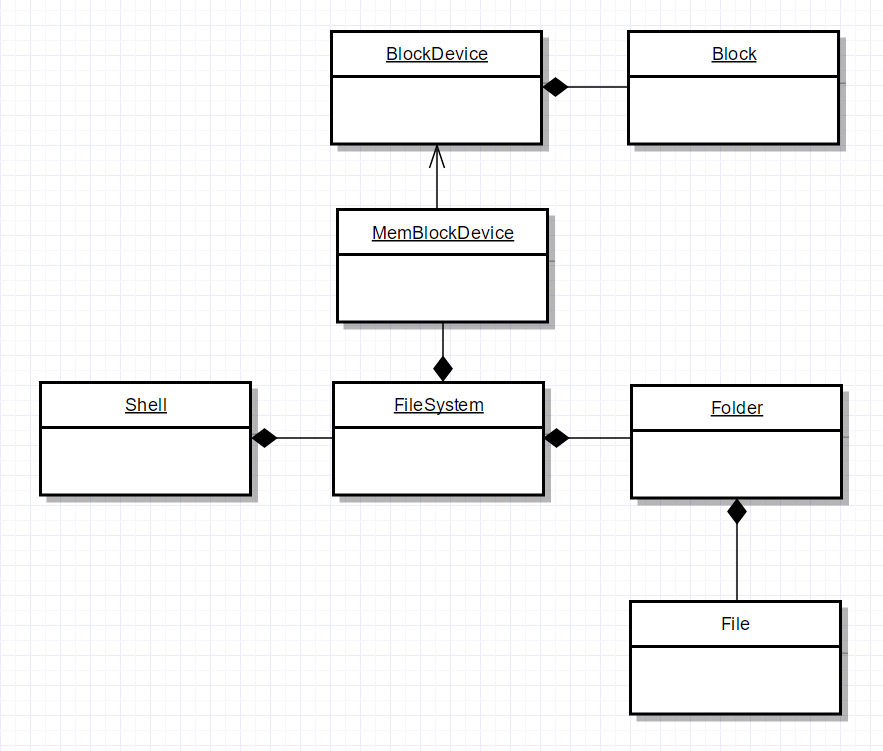
\includegraphics[width=7cm]{klassdiagram.png}
		\caption{Klassdiagram över alla klasser i projektet}
	\end{center}
\end{figure}

\subsection{Resultat}
Alla funktioner för betyget E blev implementerat. Se bifogade C++ filer för källkod.


\section{Avslutande}
\subsection{Slutsats}
Uppgiften var väl skapad för att ge laboranterna en djupare förståelse för filsystem och de vanligaste problemen ett man kan stöta på när man skapar ett format av filsystem. Vi lärde oss mycket om hanteringen av mapporganisation och svårigheterna med att kunna spara data på ett optimalt sätt. 

\subsection{Tidsredovisning}
Implementationen av filsystemet tog ca. 40 timmar och rapporten är skriven på 6 timmar.

\begin{thebibliography}{3}

	\bibitem{bok 1}
		Tanenbaum,A.S., Bos,H., \textit{Modern Operating Systems}, Upplaga $4$, Global Edition, $2015$.
		
	\bibitem{bok 2}
		Nilsson, Carina, \textit{Introduktion till Linux}, Blekinge Tekniska Högskola, $2016$.
		
		\bibitem{bok 3}
		Nilsson, Carina, Phung, Cuong \textit{Projekt – Simulering av filsystem}, Blekinge Tekniska Högskola, $2016$.

\end{thebibliography}

\end{document}
